\section{Vergleich verschiedener Algorithmen}\label{s.Ergebnisse}\raggedbottom

\subsection{Wahl der Parameter}

\subsubsection{Vergleich der drei Euklid Varianten}\label{s.keuclid}
\begin{figure}[h!]
	\centering
	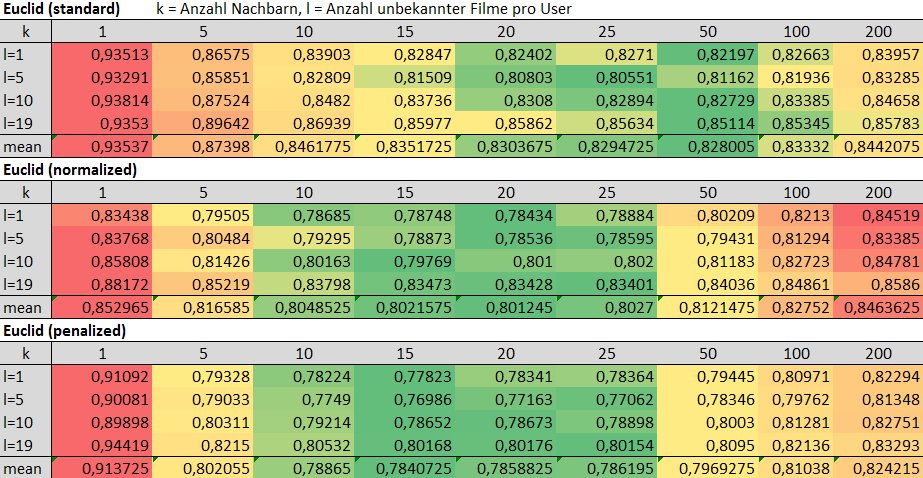
\includegraphics[width=1\linewidth]{ErrorEuclid}
	\caption{MAE im Euklid Algorithmus in Abhängigkeit der Parameter}
	\label{fig:ErrorEuclid}
	
\end{figure}
Die Werte sind mit einer Farbskala von Rot über Gelb nach Grün je Zeile formatiert, um den maximalen Fehler (rot) und den minimalen Fehler (grün) in einem Szenario besser erkennen zu können.\\\\
Wie man an den Tabellen sehen kann, verbessert die Normalisierung den Standard-Euklid-Algorithmus aus \autoref{euclid} . Eine stärkere Verbesserung wird jedoch durch die eingebaute Strafe erzielt. Mit den Parametern $k = 15$ und der Strafe kann der Fehler minimiert werden. In den folgenden Vergleichen werden immer diese Parameter benutzt.
\clearpage

\subsubsection{Wahl von $k$ bei den kNN im Pearson Algorithmus}\label{s.kpearson}
\begin{figure}[h!]
\centering
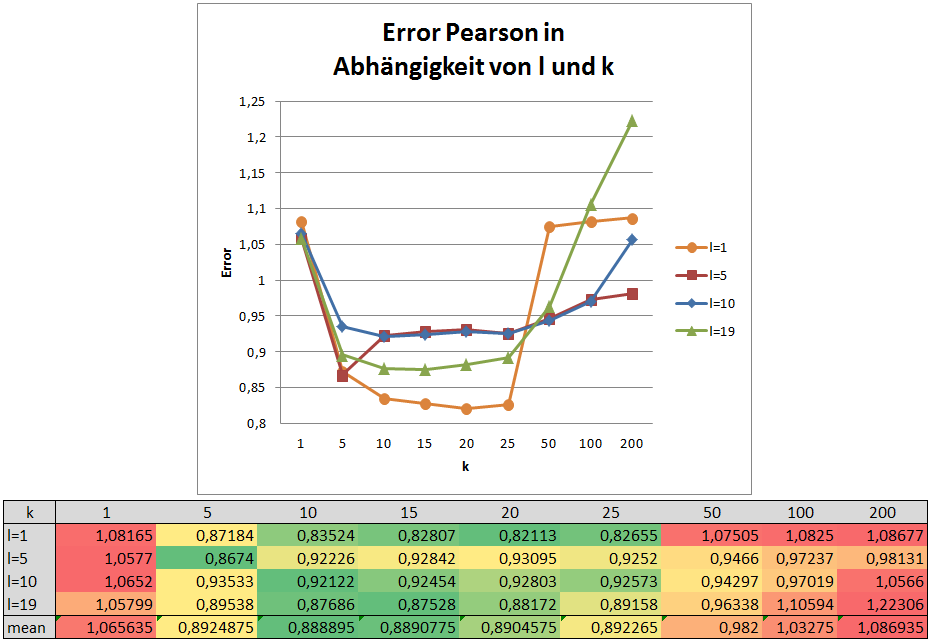
\includegraphics[width=1\linewidth]{ErrorPearsonk}
\caption{MAE im Pearson Algorithmus in Abhängigkeit der Parameter }
\label{fig:ErrorPearsonk}
\end{figure}
Eine Wahl von $k = 10$ nächsten Nachbarn optimiert den Pearson Algorithmus. Im Szenario $l = 1$ zeigt der Algorithmus seine Stärken. Wenn viele Informationen vorhanden sind, können mit dem Pearson Algorithmus gute Bewertungen vorhergesagt werden. Wenn man die mittleren Szenarien $l = 5$ und $l = 10$ mit $l = 19$ vergleicht, fällt auf, dass das letzte Szenario am besten abschneidet. Da hier 19 Fehler berechnet und gemittelt werden. Im Fall $l = 5$ werden nur fünf Fälle verglichen, dadurch entsteht im Mittel eine größere Abweichung zwischen der Vorhersage und der tatsächlich abgegeben Bewertung.
\clearpage

\subsubsection{Wahl von $k$ bei den kNN im Floyd Warshall Algorithmus}\label{s.kflowar}
\begin{figure}[h!]
\centering
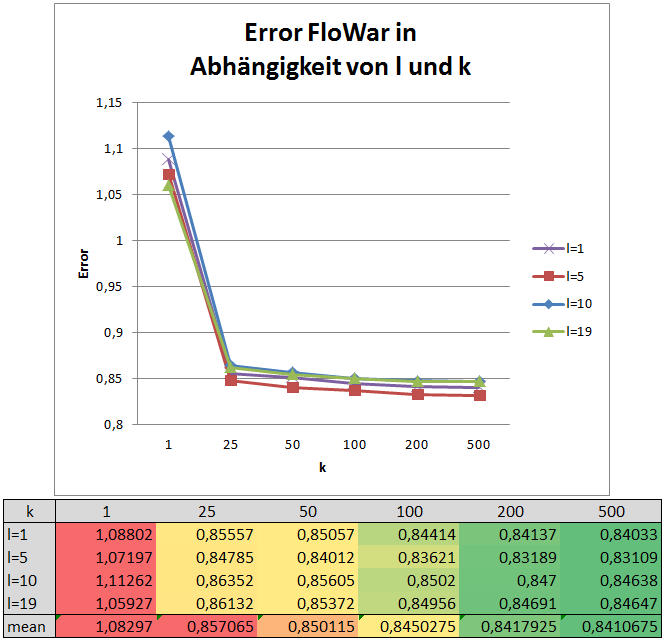
\includegraphics[width=1\linewidth]{ErrorFloWark}
\caption{MAE im Floyd Warshall Algorithmus in Abhängigkeit der Parameter}
\label{fig:ErrorFloWark}
\end{figure}
Man sieht in \autoref{fig:ErrorFloWark}, dass Floyd-Warshall bei großem $k$ (=500) am besten funktioniert. Es wird das Minimum aus den $k$ nächsten Nachbarn und den $n$ nächsten Nachbarn, die den aktuell zu bewertenden Film überhaupt bewertet haben, genommen, um das zu erwartete Rating zu ermitteln. Dies tendiert gegen den Durchschnittswert aller User, die die fehlenden Items bewertet haben. Somit ist der FW-Algorithmus fast gleichzusetzen mit dem Itemmean.
\clearpage

\subsubsection{Wahl von $a$ beim Hybrid Algorithmus}\label{s.alugu}

\begin{figure}[h!]
\centering
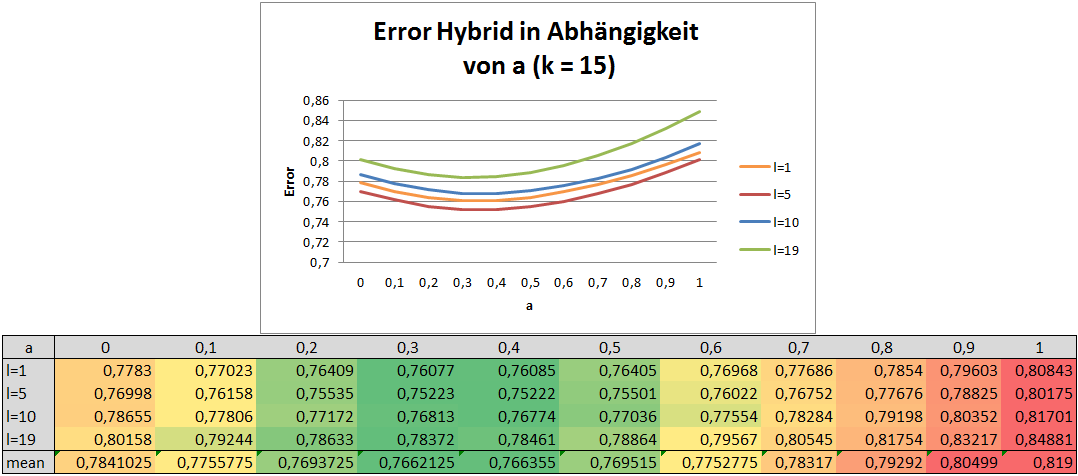
\includegraphics[width=1\linewidth]{ErrorHybrida}
\caption{MAE im Hybrid Algorithmus in Abhängigkeit der Parameter}
\label{fig:ErrorLUSGUSa}
\end{figure}
\FloatBarrier
Ein Verhältnis aus 70\% Euklid und 30\% Slope One minimiert den Fehler. Während der Euklid Algorithmus nur ähnliche Nachbarn untersucht, hilft das Wissen aus dem Item-basierten Algorithmus Slope One den MAE weiter zu minimieren.


\subsection{Auswertung der Fehlerberechnung}\label{s.auswertung}
Neben den sechs genannten Algorithmen (s. \nameref{tab:Liste der Algorithmen}) habe ich noch drei weitere Algorithmen für den Vergleichstest implementiert. Der einfachste, Random, erzeugt einen randomisierten Float zwischen $[1,5]\subset \mathbb{R}$. Usermean $\bar{R}^{user}_{u}$ ermittelt den Durchschnitt des Users, der gerade betrachtet wird. Itemmean $\bar{R}^{item}_{i}$ berechnet die durchschnittliche Bewertung aller User des Items, das gerade im Fokus ist (s. \autoref{definition}). 
Gegen diese drei simplen Algorithmen werden die MAE der sechs oben beschriebenen Funktionen gemessen. Wobei wieder alle vier Szenarien bezüglich des Parameters $l$ betrachtet werden.\\

\begin{figure}[h!]
\centering
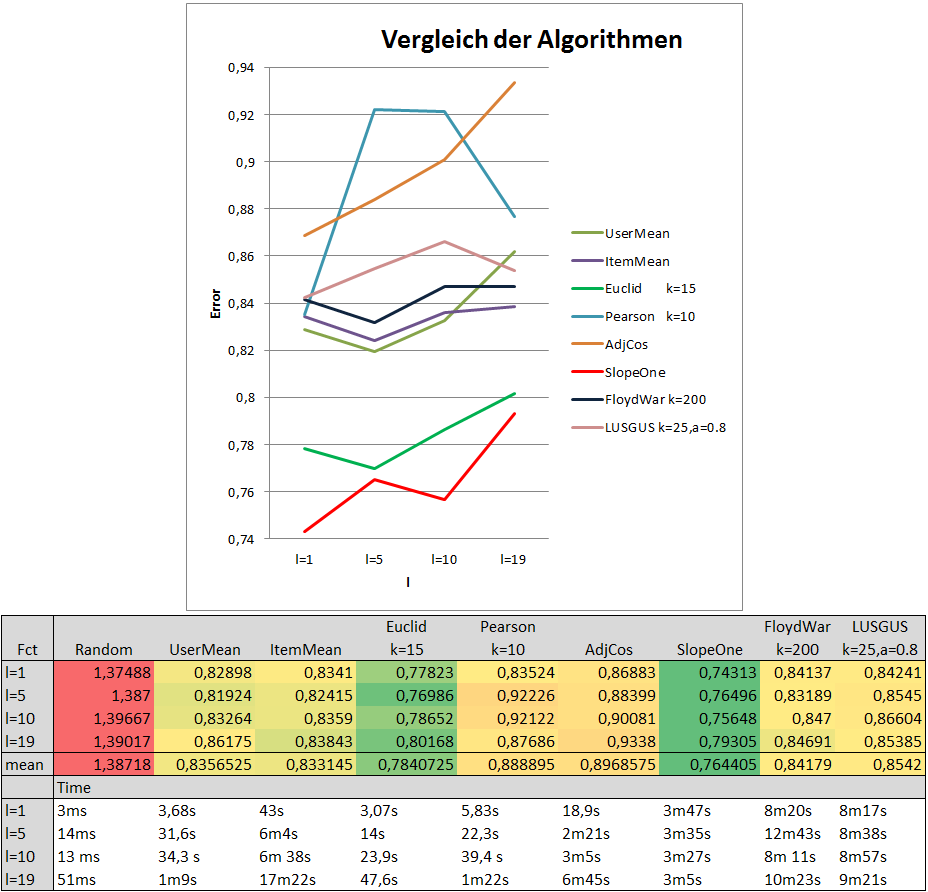
\includegraphics[width=1\linewidth]{Vergleich}
\caption{MAE Vergleich aller Algorithmen}
\label{fig:Vergleich}
\end{figure}
\FloatBarrier
Die Laufzeiten dienen als zusätzlicher Vergleich zwischen den Algorithmen. Die Daten sind in einer Hashmap gespeichert und es wird nur ein Kern der CPU ausgelastet. Durch andere Implementierungen und andere PC-Setups können die Zeiten variieren.\\
Usermean und Itemmean erzielen im Vergleich kein schlechtes Ergebnis, zählen sogar laut MAE mit zu den besten Algorithmen. Usermean ist für Vorhersagen nicht brauchbar, da jedes unbekannte Item das gleiche Rating bekommt. Einen Einsatz findet dieser Algorithmus nur, wenn kein anderer User diesen Film bisher bewertet hat. Bei Itemmean können zwar allgemein beliebte Filme vorgeschlagen werden, die Vorlieben des Users werden aber komplett ignoriert. Pearson erkennt sogar Ähnlichkeiten in relativen Abweichungen und kommt somit mit einem geringem $k$ im k-Nearest-Neighbors aus. Das genaue Gegenteil ist bei Floyd-Warshall der Fall. Der sehr groß eingestellte Parameter $k$ führt dazu, dass FW ähnlich wie Itemmean die bekannten Informationen über den User vernachlässigt. Da mit dem Itemmean eine bessere durchschnittliche Abweichung erzielt wird, als über die entdeckten Pfade zu anderen User. Adjusted Cosine Similarity ist in diesem Test nicht sehr erfolgreich. Obwohl es mit dem gleichen Score arbeitet wie der PCC und dort alle bekannten Informationen über die zwei Items verwendet, können keine guten Vorhersagen erzielt werden. Bessere Vorhersagen erzielt man  mit dem Item-basierten Algorithmus Slope One. Die absolute durchschnittliche Differenz zwischen den Items verwendet alle verfügbaren Informationen aus dem Datensatz. Neben den Differenzen zwischen allen Items muss auch noch eine Frequenzmatrix gespeichert werden. Neue Informationen können dadurch ohne großen Rechenaufwand in die Abstandsmatrix eingearbeitet werden. Die Vorberechnungen im Slope One machen allerdings nur ca. 30 Sekunden der gesamten Zeit aus. Damit braucht der Algorithmus auch recht lange, um Vorhersagen für viele Nutzer gleichzeitig zu berechnen. Der Algorithmus mit dem euklidischen Abstand und Strafe schneidet sehr gut ab und hat dazu sehr kurze Berechnungszeiten. Ein noch besseres Ergebnis liefert das Hybrid Verfahren. Das gemittelte Rating zu 70\% aus dem besten User-basierten (Euklid mit Strafe) und zu 30\% aus dem besten Item-basierten Algorithmus (Slope One) minimiert in diesem Test den MAE. Jedoch verlängert Slope One die Laufzeit immens.\\

\begin{figure}[h!]
	\centering
	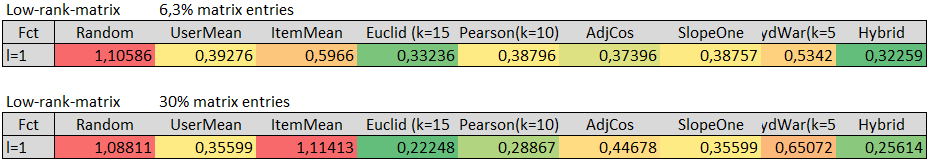
\includegraphics[width=1\linewidth]{bilder/lowrank}
	\caption{MAE Vergleich mit einer Matrix mit niedrigem Rang}
	\label{fig:LowRankMatrix}
\end{figure}
\FloatBarrier
Bei der Konstruktion mit niedrigem Rang erkennt man, dass die User-basierten Algorithmen richtig gut werden. Das ist aber auch zu erwarten, denn die User ähneln sich sehr stark, da sie alle aus einer Kombination aus dreißig Basis-Usern entstanden sind. Die Bewertungen wurden zufällig erstellt, dadurch können auch keine Ähnlichkeiten zwischen den Filmen entstehen. Dies wertet die Item-basierten Algorithmen zusätzlich ab. Sind viele Informationen bekannt, ändert sich nicht viel an der Reihenfolge der Algorithmen.\\
Einen Vergleich zu der realen Datenbank von MovieLens kann man nur mit Vorsicht tätigen. Wenn man die Histogramme der beiden Matrizen betrachtet, wird klar, dass die Konstruktion der Matrix mit niedrigem Rang nicht sehr nah an die Verteilung der MovieLens-Daten heran kommt.
\begin{figure}[h!]
	\centering
	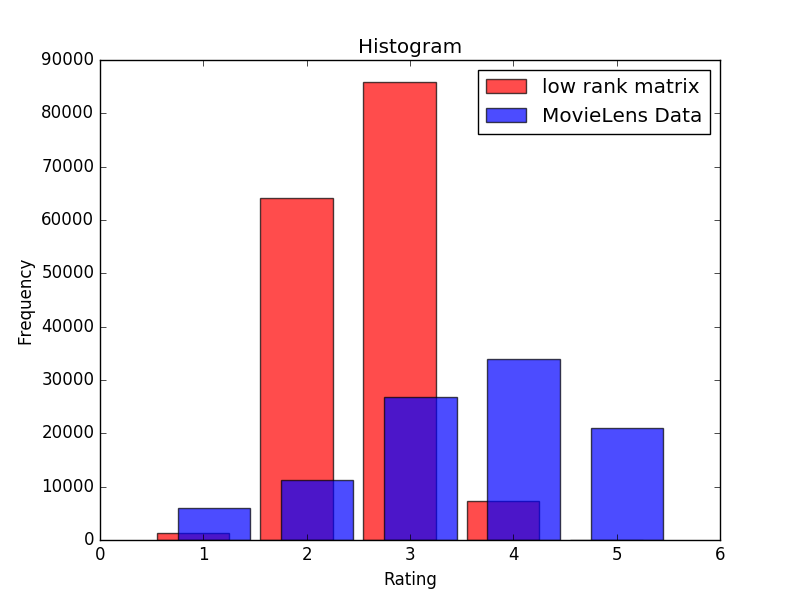
\includegraphics[width=1\linewidth]{histogram}
	\caption{Histogramm Vergleich}
	\label{fig:histogram}
\end{figure}
\FloatBarrier
Beim Versuch die Bewertungen gleichmäßiger zu verteilen, zerstört man die lineare Abhängigkeit der Zeilen. Doch genau diese Eigenschaft der Bewertungen wollte ich mit diesem Test überprüfen. Überraschend ist die Verteilung der MovieLens-Daten. Ich hätte erwartet, dass die 1 häufiger von enttäuschten Usern als negative Bewertung benutzt wird.

\begin{figure}[h!]
	\centering
	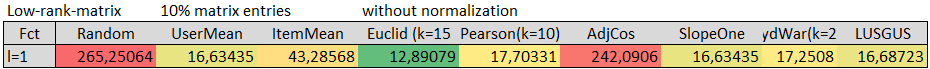
\includegraphics[width=1\linewidth]{lowranknotnorm}
	\caption{MAE Vergleich ohne Normalisierung}
	\label{fig:LowRankMatrixnotnorm}
\end{figure}
\FloatBarrier
In den Daten in \autoref{fig:LowRankMatrixnotnorm} wurde bewusst vermieden, die Bewertungen wieder in den Wertebereich ${1,2,3,4,5}$ zu normieren. Dadurch wird die lineare Abhängigkeit der Zeilen nicht zerstört. Diese erzielten Fehler können deshalb nicht mit den anderen Szenarien verglichen werden. Was man aber erkennen kann, dass die User-basierten Verfahren sehr viel besser abschneiden, als der Item-basierte Algorithmus Adjusted Cosine Similarity. Slope One kann auch hier mit den vollen Informationen der Matrix ein sehr gutes Ergebnis erzielen.
\clearpage